\documentclass[a4paper]{article}
\linespread{1.6}
\usepackage{geometry}
\usepackage{setspace}
\usepackage{amsmath}
\usepackage{amssymb}
\usepackage{enumerate}
\usepackage[pdftex]{graphicx}
\usepackage{float}
\usepackage{subfigure}
\usepackage{listings}
\geometry{left=1.5cm,right=1.5cm,top=2.5cm,bottom=2.5cm}

\begin{document}
\begin{spacing}{2.0}
\begin{flushleft}\begin{huge}EEE5502 Foundations of Digital Signal Processing   Code 7\end{huge}\end{flushleft}
\begin{flushright}\begin{Large} Hudanyun Sheng \end{Large}\end{flushright}

\Large\textbf{ Question \#1}:  \\
\normalsize
I spent 2 hours.\\

\Large\textbf{Question \#2}:  \\
\normalsize
I add another variable $\lambda$ as an input to the function ``sift\_func.mat", and the window size $W$ is set to be 1000, $\lambda$ is set to be 0.9.\\
The image of the STFT before and after the spectral subtraction processing is shown below, we can observe that before spectral subtraction processing, there is a lot noise, the spectral subtraction processing gets rid of them. 
\begin{figure} [H]
\centering
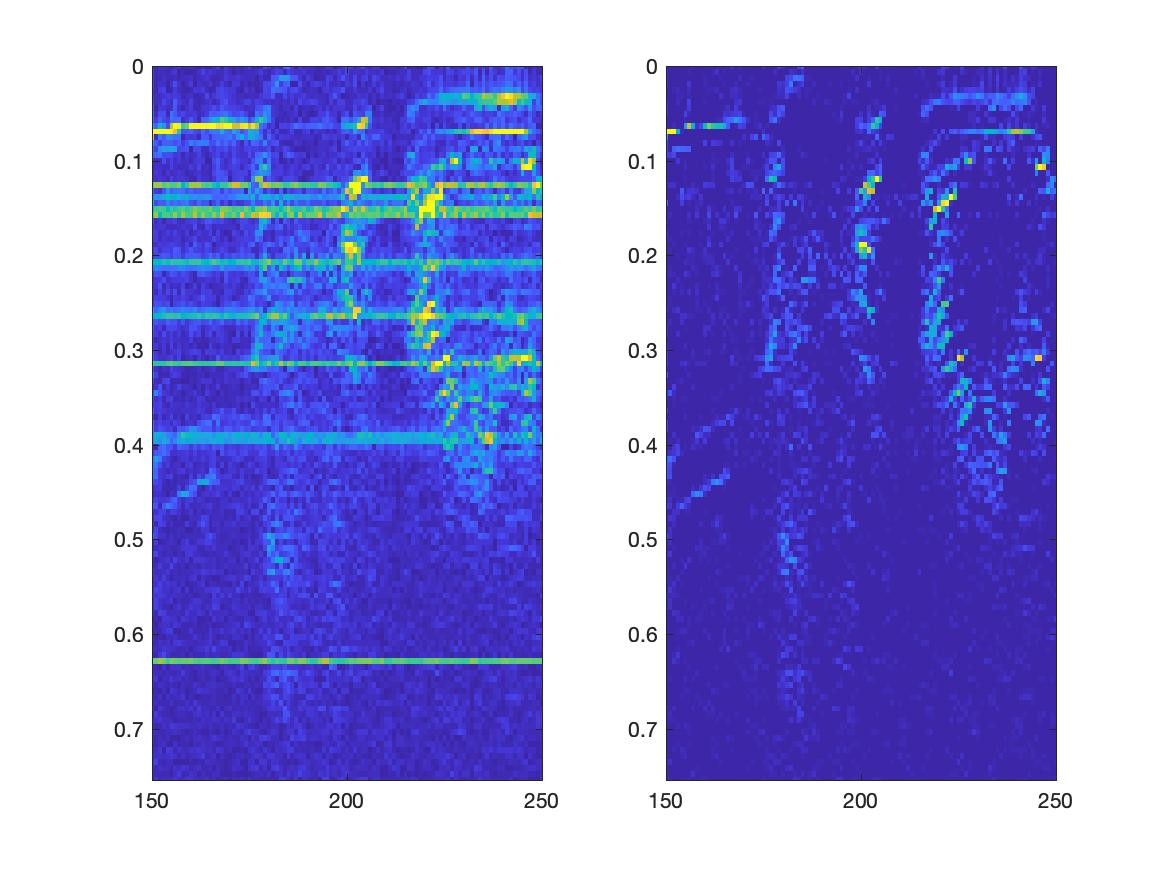
\includegraphics[width=4in]{1.jpg}
\label{fig:graph}
\end{figure}

The original speech and the reconstructed noise-free audio is shown in the plot below:
\begin{figure} [H]
\centering
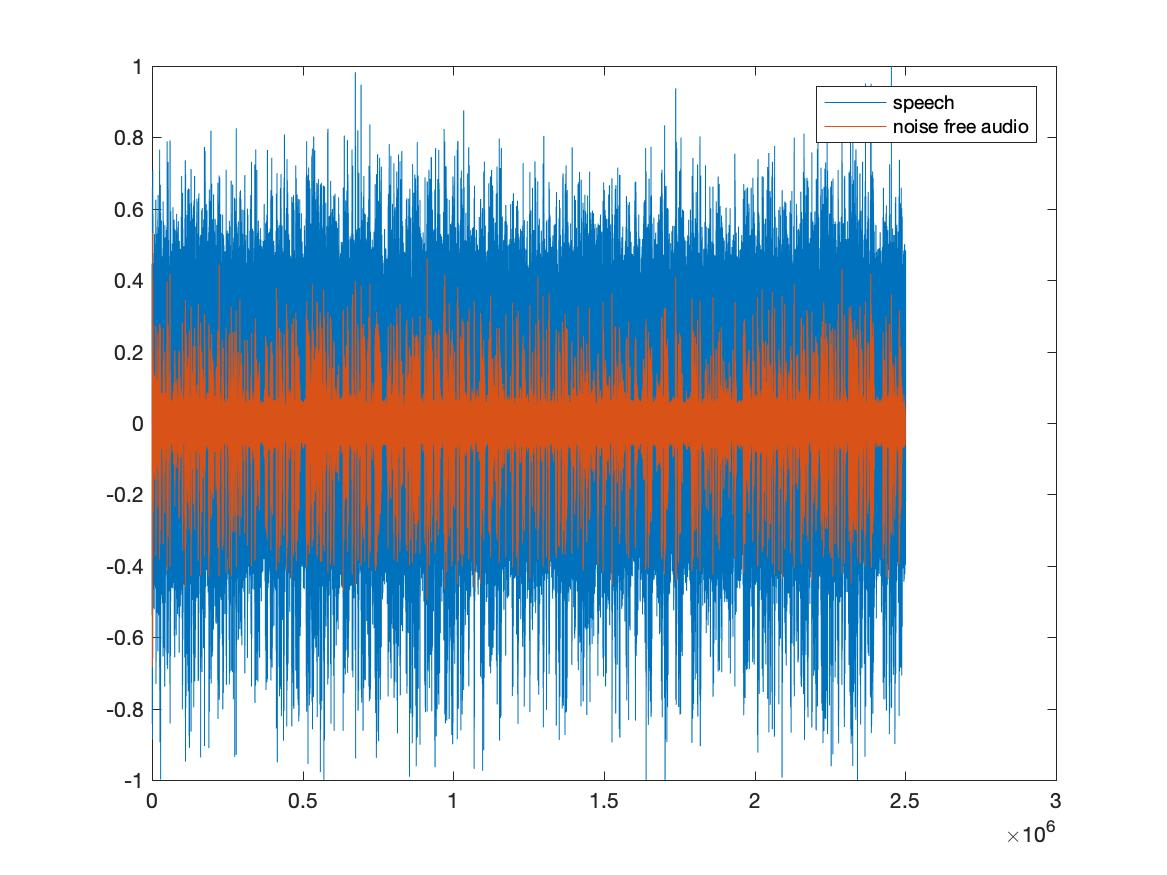
\includegraphics[width=4in]{1_audio.jpg}
\label{fig:graph}
\end{figure}








\end{spacing}
\end{document}